\section{Requisiti soddisfatti}\label{section:requisiti_soddisfatti}
Secondo quanto riportato nel \docNameVersionPdP{}, il gruppo \groupName{} è riuscito a soddisfare tutti i requisiti obbligatori.
Arrivati a questo punto si è avviata anche la codifica delle funzionalità opzionali e desiderabili che proseguirà nel periodo successivo.
\subsection{Tabella requisiti soddisfatti}
Segue una tabella con l'elenco di tutti i requisiti funzionali soddisfatti.

\begin{table}[H]
    \centering
    \renewcommand{\arraystretch}{1.8}
    \rowcolors{2}{green!100!black!40}{green!100!black!30}
    \begin{tabular}{c | c | p{6cm} | c }
        \rowcolor[HTML]{125E28}
        \multicolumn{1}{c}{\color[HTML]{FFFFFF} \textbf{Codice}}          &
        \multicolumn{1}{c}{\color[HTML]{FFFFFF} \textbf{Classificazione}} &
        \multicolumn{1}{c}{\color[HTML]{FFFFFF} \textbf{Descrizione}}     &
        \multicolumn{1}{c}{\color[HTML]{FFFFFF} \textbf{Stato}}                                                                                                                                                                  \\
        \hline
        R1F1                                                              & Obbligatorio & Si deve processare una richiesta di checkout da un e-commerce\glo{}.                          & Soddisfatto                        \\
        R1F2                                                              & Obbligatorio & L'utente deve poter scegliere la tipologia di pagamento.                                      & Soddisfatto        \\
        R1F2.1                                                            & Obbligatorio & L'utente deve poter scegliere la tipologia di pagamento unico.                                & Soddisfatto      \\
        R2F2.2                                                            & Desiderabile & L'utente deve poter scegliere la tipologia di pagamento MoneyBox\glo{}.                       & Soddisfatto      \\
        R2F2.2.1                                                          & Desiderabile & Si deve poter visualizzare lo stato di completamento della MoneyBox\glo{}.                    & Soddisfatto                                 \\
        R2F2.2.2                                                          & Desiderabile & Si deve poter copiare l’invito di partecipazione alla MoneyBox\glo{}.                         & Soddisfatto                                 \\
        R3F2.2.3                                                          & Opzionale    & L'utente deve poter visualizzare una traduzione visiva dell'indirizzo MoneyBox\glo{}.         & Non Soddisfatto        \\
        R2F2.2.4                                                          & Desiderabile & Si deve poter chiudere la MoneyBox\glo{} restituendo i soldi.                                 & Soddisfatto                                  \\
        R2F2.2.5                                                          & Desiderabile & L'utente deve poter visualizzare l'elenco delle transazioni partecipanti alla MoneyBox\glo{}. & Soddisfatto \\
        R1F3                                                              & Obbligatorio & L'utente deve poter visualizzare il totale dell'ordine.                                       & Soddisfatto \\
        R1F4                                                              & Obbligatorio & L'utente deve poter effettuare la connessione a Metamask\glo{}.                               & Soddisfatto   \\
        R1F5                                                              & Obbligatorio & L'utente deve poter pagare.                                                                   & Soddisfatto \\
    \end{tabular}
\end{table}
\begin{center}
    \textit{\small Continua nella pagina successiva}
\end{center}
\begin{table}[H]
    \centering
    \renewcommand{\arraystretch}{1.8}
    \rowcolors{2}{green!100!black!40}{green!100!black!30}
    \begin{tabular}{c | c | p{6cm} | c}
        \rowcolor[HTML]{125E28}
        \multicolumn{1}{c}{\color[HTML]{FFFFFF} \textbf{Codice}}          &
        \multicolumn{1}{c}{\color[HTML]{FFFFFF} \textbf{Classificazione}} &
        \multicolumn{1}{c}{\color[HTML]{FFFFFF} \textbf{Descrizione}}     &
        \multicolumn{1}{c}{\color[HTML]{FFFFFF} \textbf{Stato}}                                                                                                                                                                                          \\
        \hline
        R1F5.1                                                            & Obbligatorio & L'utente che ha scelto il metodo di pagamento unico deve pagare interamente la somma richiesta.                       & Soddisfatto      \\
        R2F5.2                                                            & Desiderabile & L'utente che partecipa al pagamento MoneyBox\glo{} deve poter pagare una parte della somma richiesta.                 & Soddisfatto      \\
        R1F5.4                                                            & Obbligatorio & L'utente deve poter visualizzare un messaggio d'errore nel caso in cui la transazione fallisca.                       & Soddisfatto                               \\
        R1F6                                                              & Obbligatorio & Il proprietario dell'ordine o il venditore devono poter richiedere il rimborso della transazione.                     & Soddisfatto   \\
        R1F7                                                              & Obbligatorio & Il proprietario dell'ordine deve poter confermare la ricezione e quindi sbloccare i fondi dallo smart contract\glo{}. & Soddisfatto   \\
        R1F7.1                                                            & Obbligatorio & Il proprietario dell'ordine deve poter visualizzare il codice di sblocco.                                             & Soddisfatto   \\
        R1F8                                                              & Obbligatorio & L'utente deve poter visualizzare le transazioni.                                                                      & Soddisfatto   \\
        R2F8.1                                                            & Desiderabile & Il venditore deve poter visualizzare le transazioni in entrata pagate.                                                & Soddisfatto \\
        R2F8.1.1                                                          & Desiderabile & Il venditore deve poter visualizzare le transazioni in entrata pagate non sbloccate.                                  & Soddisfatto                              \\
        R2F8.1.2                                                          & Desiderabile & Il venditore deve poter visualizzare le transazioni in entrata pagate e sbloccate.                                    & Soddisfatto                               \\
        R2F8.1.3                                                          & Desiderabile & Il venditore deve poter visualizzare le transazioni in entrata pagate ma cancellate.                                  & Soddisfatto                               \\
        R1F8.2                                                            & Obbligatorio & Il proprietario dell'ordine deve poter visualizzare le transazioni in uscita.                                         & Soddisfatto                                 \\
    \end{tabular}
\end{table}
\begin{center}
    \textit{\small Continua nella pagina successiva}
\end{center}
\begin{table}[H]
    \centering
    \renewcommand{\arraystretch}{1.8}
    \rowcolors{2}{green!100!black!40}{green!100!black!30}
    \begin{tabular}{c | c | p{6cm} | c}
        \rowcolor[HTML]{125E28}
        \multicolumn{1}{c}{\color[HTML]{FFFFFF} \textbf{Codice}}          &
        \multicolumn{1}{c}{\color[HTML]{FFFFFF} \textbf{Classificazione}} &
        \multicolumn{1}{c}{\color[HTML]{FFFFFF} \textbf{Descrizione}}     &
        \multicolumn{1}{c}{\color[HTML]{FFFFFF} \textbf{Stato}}                                                                                                                                                                  \\
        \hline
        R2F8.2.1                                                          & Desiderabile & Il proprietario dell'ordine deve poter visualizzare le transazioni in uscita non pagate.                   & Soddisfatto                  \\
        R2F8.2.2                                                          & Desiderabile & Il proprietario dell'ordine deve poter visualizzare le transazioni in uscita pagate ma non sbloccate.      & Soddisfatto                  \\
        R2F8.2.3                                                          & Desiderabile & Il proprietario dell'ordine deve poter visualizzare le transazioni in uscita pagate e sbloccate.           & Soddisfatto                  \\
        R2F8.2.4                                                          & Desiderabile & Il proprietario dell'ordine deve poter visualizzare le transazioni in uscita cancellate.                   & Soddisfatto                  \\
        R3F9                                                              & Opzionale    & Si deve convertire l'ammontare depositato sullo smart contract\glo{} in stable coin\glo{}.                 & Non Soddisfatto               \\
        R3F10                                                             & Opzionale    & La piattaforma deve trattenere una piccola somma in percentuale di un ordine destinata al fondo ShopChain. & Non Soddisfatto \\
        R1F11                                                             & Obbligatorio & L'utente deve poter visualizzare il suo indirizzo wallet\glo{}.                                                  & Soddisfatto                      \\
        R1F11.1                                                           & Obbligatorio & L'utente deve poter visualizzare il suo indirizzo wallet\glo{} in forma testuale.                                & Soddisfatto                    \\
        R1F11.2                                                           & Obbligatorio & L'utente deve poter visualizzare un avviso della mancata connessione a Metamask\glo{}.                     & Soddisfatto                    \\
        R3F11.3                                                           & Opzionale    & L'utente deve poter visualizzare il suo indirizzo wallet\glo{} sotto forma di stringa di emoji.                  & Non Soddisfatto                    \\
        R3F12                                                             & Opzionale    & Gli utenti partecipanti devono ricevere una notifica al completamento della MoneyBox\glo{}.                & Non Soddisfatto \\
    \end{tabular}
\end{table}
\begin{center}
    \textit{\small Continua nella pagina successiva}
\end{center}
\begin{table}[H]
    \centering
    \renewcommand{\arraystretch}{1.8}
    \rowcolors{2}{green!100!black!40}{green!100!black!30}
    \begin{tabular}{c | c | p{6cm} | c}
        \rowcolor[HTML]{125E28}
        \multicolumn{1}{c}{\color[HTML]{FFFFFF} \textbf{Codice}}          &
        \multicolumn{1}{c}{\color[HTML]{FFFFFF} \textbf{Classificazione}} &
        \multicolumn{1}{c}{\color[HTML]{FFFFFF} \textbf{Descrizione}}     &
        \multicolumn{1}{c}{\color[HTML]{FFFFFF} \textbf{Stato}}                                                                                                                                                                   \\
        \hline
        R1F14                                                             & Obbligatorio & L'utente deve poter visualizzare lo stato di connessione a Metamask\glo{}.                                       &Soddisfatto                      \\
        R1F14.1                                                           & Obbligatorio & L'utente deve poter visualizzare una conferma di connessione corretta a Metamask\glo{}.                      & Soddisfatto                     \\
        R1F14.2                                                           & Obbligatorio & L'utente deve poter visualizzare un errore nel caso non sia installato Metamask\glo{}.                                             & Soddisfatto   \\
        R1F14.3                                                           & Obbligatorio & L'utente deve poter visualizzare un errore nel caso in cui la blockchain selezionata non sia corretta.                       & Soddisfatto   \\
        R1F14.4                                                           & Obbligatorio & L'utente deve poter visualizzare un errore nel caso in cui non abbia connesso un account a ShopChain.                        & Soddisfatto   \\
        R1F15                                                             & Obbligatorio & L'utente deve poter visualizzare un messaggio di avviso nel caso in cui la transazione sia già presente in blockchain\glo{}. & Soddisfatto \\
        R1F16                                                             &Obbligatorio  & L'utente deve poter visualizzare una pagina con i dettagli dell' ordine pagato.                                               & Soddisfatto\\
        R1F16.1                                                           & Obbligatorio & L'utente deve poter visualizzare i dettagli dell'ordine pagato.                                                              & Soddisfatto   \\ 
        R1F16.1.1                                                           & Obbligatorio & L'utente deve poter visualizzare l'id dell'ordine pagato.                                                                    & Soddisfatto \\ 
        R1F16.1.2                                                           & Obbligatorio & L'utente deve poter visualizzare l'indirizzo del venditore dell'ordine pagato.                                               & Soddisfatto \\ 
        R1F16.1.3                                                           & Obbligatorio & L'utente deve poter visualizzare l'ammontare dell'ordine pagato.                                                             & Soddisfatto \\ 
        R1F16.1.4                                                           & Obbligatorio & L'utente deve poter visualizzare lo stato dell'ordine pagato.                                                                & Soddisfatto \\ 
        R1F16.1.5                                                           & Obbligatorio & L'utente deve poter visualizzare la data dell'ordine pagato.                                                                 & Soddisfatto \\
    \end{tabular}
    \caption{Requisiti funzionali}
\end{table}


\subsection{Grafici requisiti soddisfatti}
Per quanto riguarda i requisiti funzionali il gruppo \groupName{} è riuscito a soddisfarne 43 su 48, arrivando ad una copertura del 90\%.
\begin{figure}[htbp]
    \begin{center}
     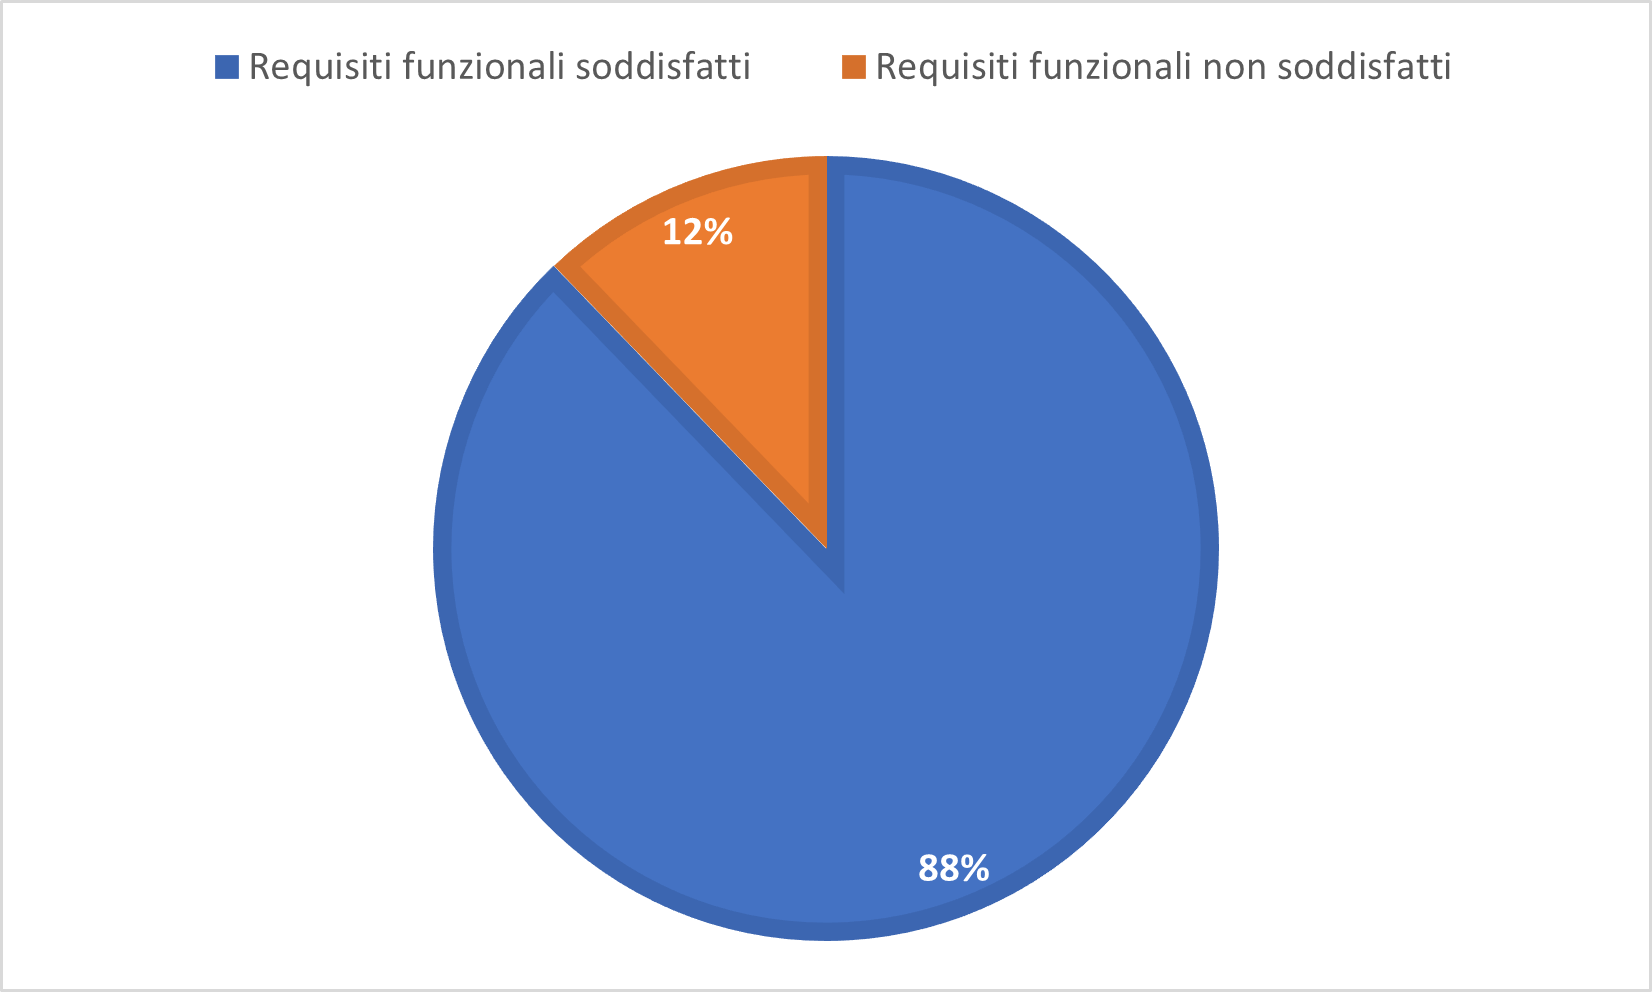
\includegraphics{immagini/requisitiFunzionali.png}
     \caption{Requisiti funzionali soddisfatti}
    \end{center}
 \end{figure}    
 

Riguardo invece i requisiti obbligatori siamo arrivati ad una copertura del 100\%.
\begin{figure}[htbp]
   \begin{center}
    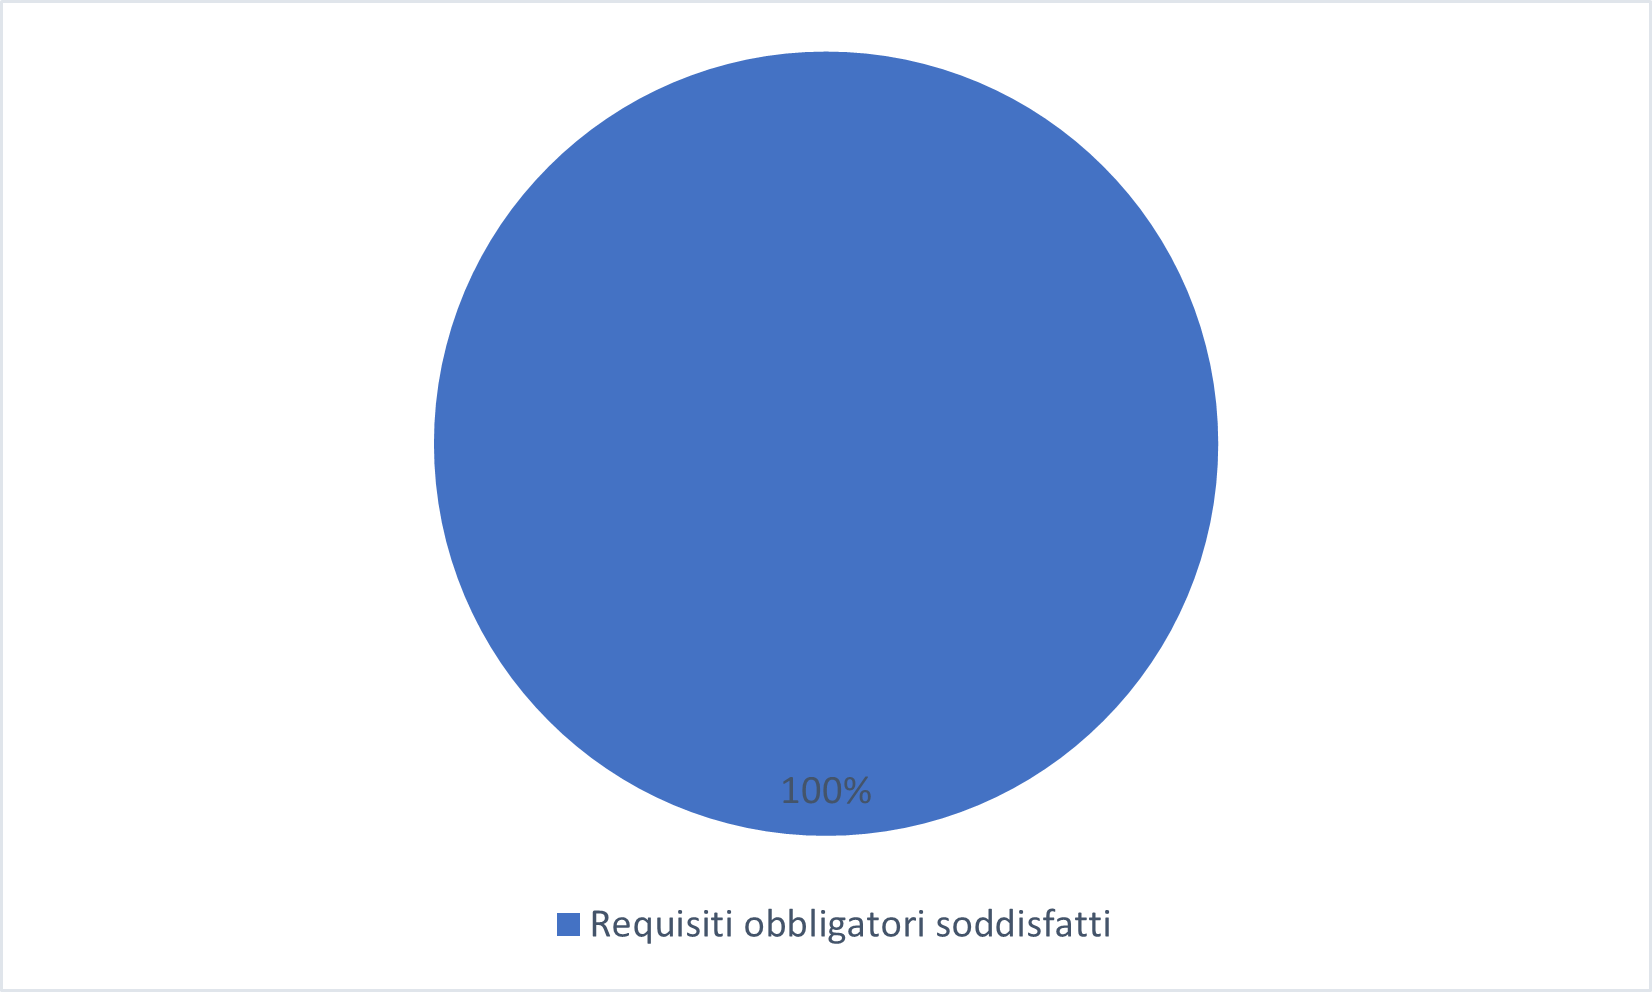
\includegraphics{immagini/requisiti_obbligatori.png}
    \caption{Requisiti obbligatori soddisfatti}
   \end{center}
\end{figure}    

